\documentclass[a4paper]{article}
\usepackage{ctex}
\usepackage[left=1.5cm, right=1.5cm, top=1.5cm, bottom=1.5cm]{geometry} %页边距
\usepackage{helvet}
\usepackage{amsmath, amsfonts, amssymb} % 数学公式、符号
\usepackage[english]{babel}
\usepackage{graphicx}   % 图片
\usepackage{url}        % 超链接
\usepackage{bm}         % 加粗方程字体
\usepackage{multirow}
\usepackage{booktabs}
\usepackage{tikz}%调用宏包tikz
\usepackage{circuitikz}%调用宏包circuitikz
\usepackage{enumerate}
\usepackage{algorithm}
\usepackage{algorithmicx}
\usepackage{algpseudocode}
\usepackage{graphicx}
\usepackage[hidelinks]{hyperref}
\usepackage{listings}
\usepackage{textcomp}
\usepackage{multicol}
\usepackage[backend=biber,style=numeric,sorting=none]{biblatex}
\addbibresource{reference.bib}

% Python listing
\newcommand\pythonstyle{\lstset{
language=Python,
basicstyle=\sffamily,
keywordstyle=\textbf,
commentstyle=\color{blue},
showstringspaces=false, 
numbers=left }}
% Python environment
\lstnewenvironment{python}[1][]{
\pythonstyle \lstset{#1} }{}

\newcommand{\threemetrics}[3]{\multirow{3}{*}{\shortstack[c]{$\textcolor{orange}{#1}$\\$\textcolor{blue}{#2}$\\$\textcolor{green}{#3}$}}}
\newcommand{\twometrics}[2]{\multirow{2}{*}{\shortstack[c]{$\textcolor{blue}{#1}$\\$\textcolor{green}{#2}$}}}

\renewcommand{\algorithmicrequire}{ \textbf{Input:}}       
\renewcommand{\algorithmicensure}{ \textbf{Output:}} 
%算法格式
\usepackage{subfigure}
\usepackage{fancyhdr} %设置页眉、页脚
\usepackage{gensymb}

\pagestyle{fancy}
\lhead{Digital Signal and Image Processing, Homework2}
\chead{}
\rhead{2024,Lab2}
\lfoot{}
\cfoot{\thepage}
\rfoot{All experiments please refer to the m file.}


\usepackage{ifthen}
\usepackage{xifthen}

\newcommand{\dom}[1]{\mathop{\mathrm{dom}}\left(#1\right)}
\newcommand{\rng}[1]{\mathop{\mathrm{rng}}\left(#1\right)}
\newcommand{\preimg}[2][]{ \ifthenelse{\isempty{#1}}
    {\mathop{\mathrm{preimage}}\left(#2\right)}
    {\mathop{\mathrm{preimage}}_{#1}\left(#2\right)} }
\newcommand{\set}[1]{\left\{#1\right\}}

\newenvironment{proof}{{\par\noindent\it Proof.}\quad\par}{\hfill $\square$\par}  

\begin{document}
\section{RGB extract and combination}
Displays as follows. From left to right, up to bottom is R,G,B.\\
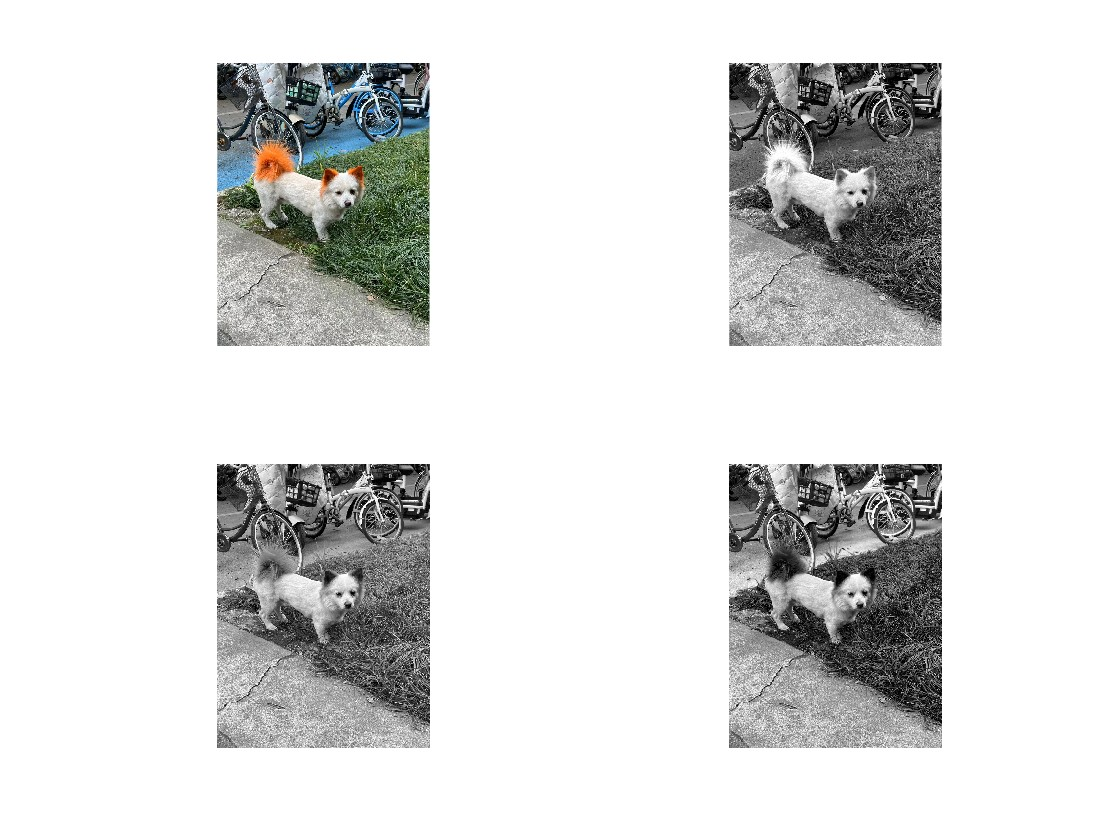
\includegraphics[scale=0.4]{figure1.jpg}\\
\centerline{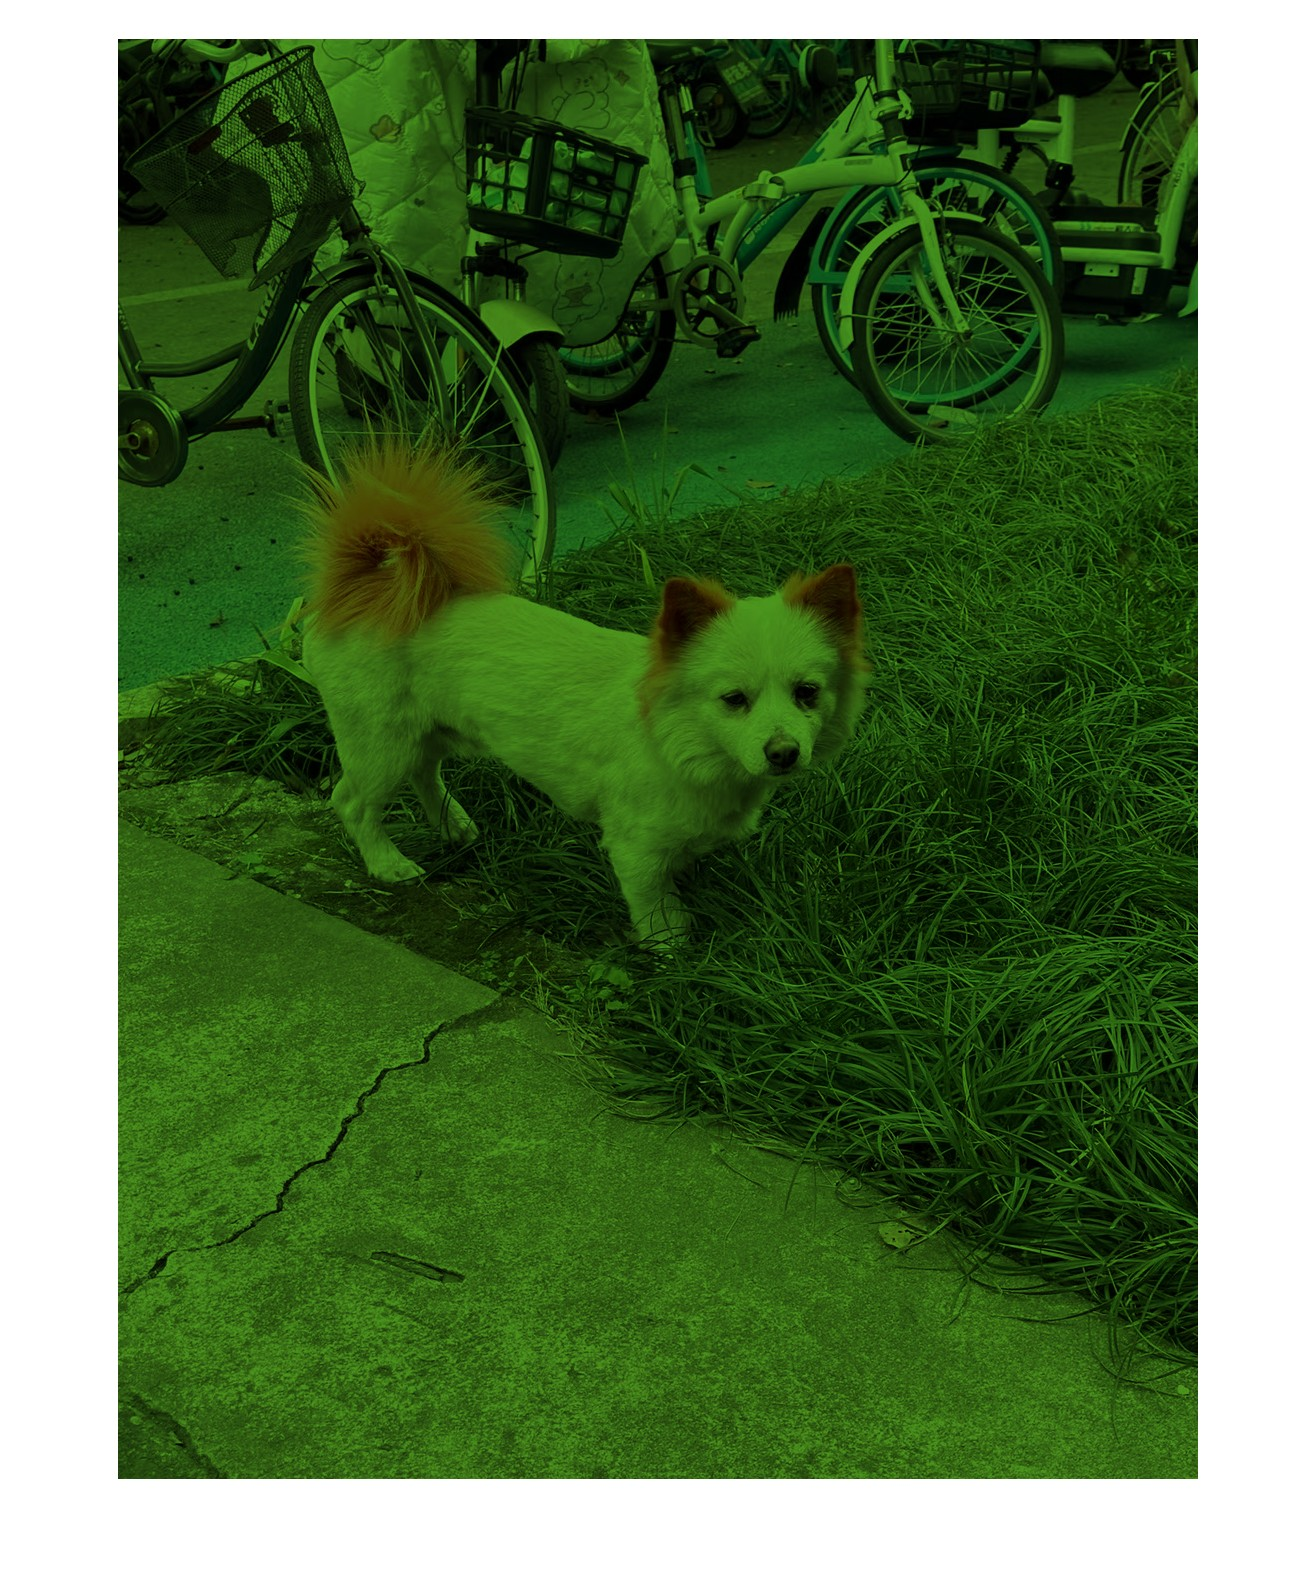
\includegraphics[scale=0.2]{figure2.jpg}}
\section{Histogram Equalization}
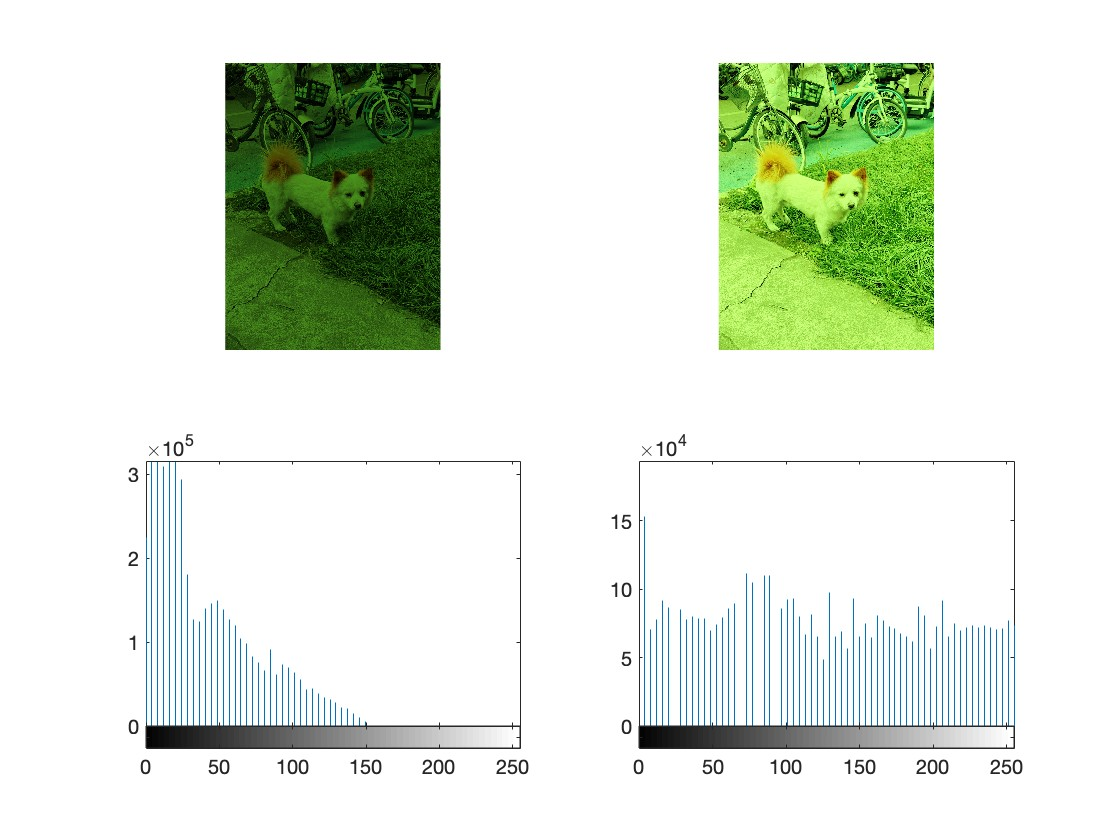
\includegraphics[scale=0.4]{figure3.jpg}
\section{Gauss Filter}
We use sigma=0.1,0.5,1,2 to implement on original image and histogram equalized image. 
Apparently histogram equalized image recovered better.\\
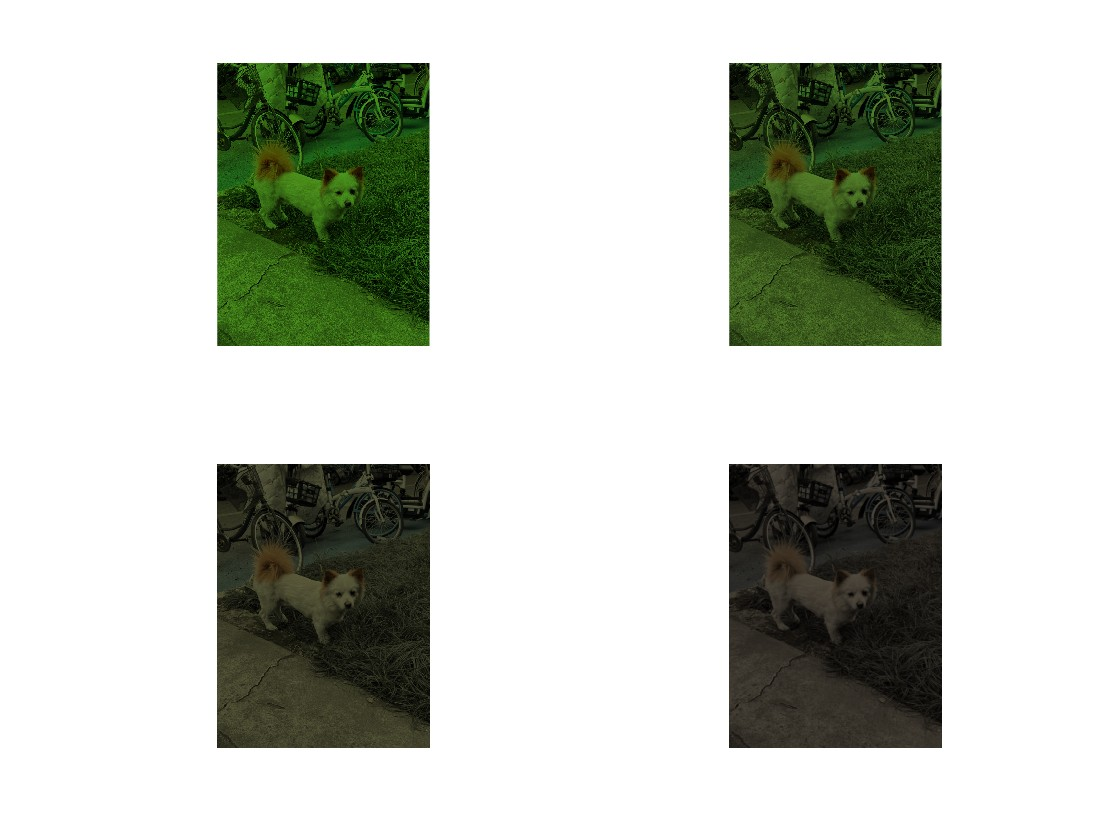
\includegraphics[scale=0.37]{figure4.jpg}
\\
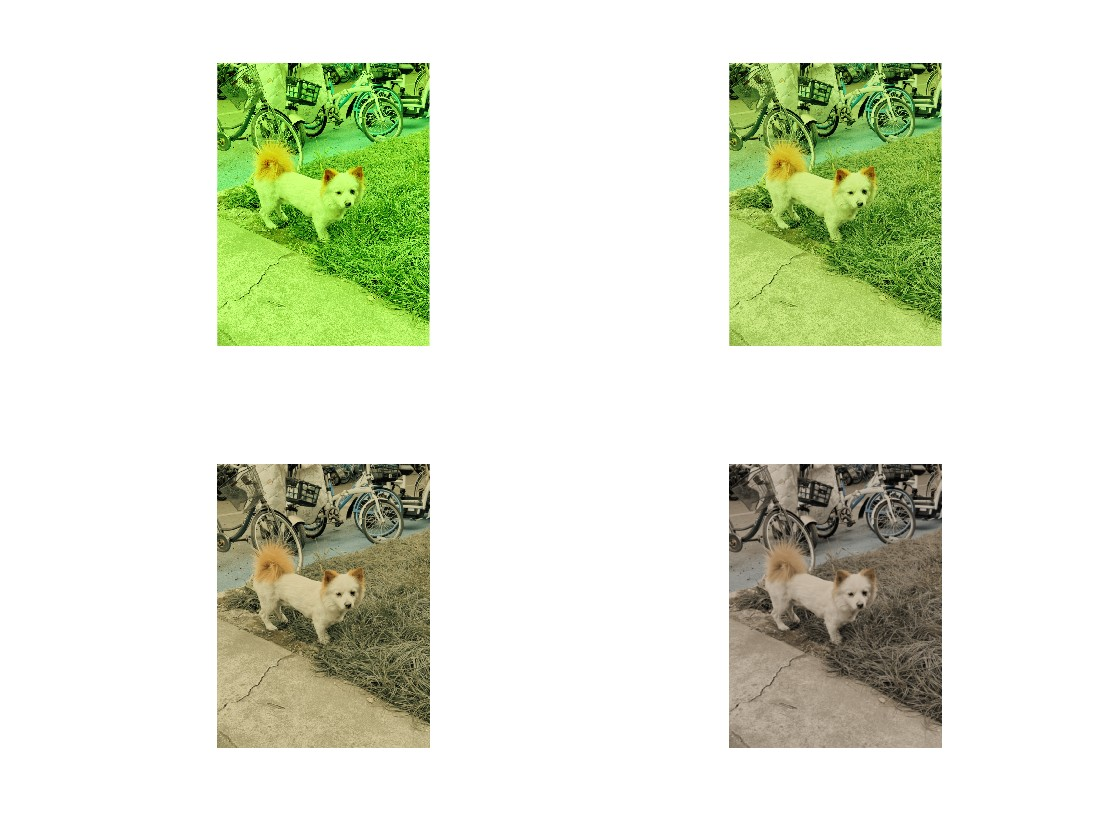
\includegraphics[scale=0.37]{figure5.jpg}
\end{document}